% ルンゲ関数の等間隔補間による比較図

\begin{figure}[H]
  \centering
  \caption{$f(x) = \frac{1}{1+25x^2}$の等間隔補間（$n=4$次多項式）}
  \label{fig:runge-equidistant-first}
  \vspace{5pt}
  \begin{minipage}[b]{0.48\linewidth}
    \centering
    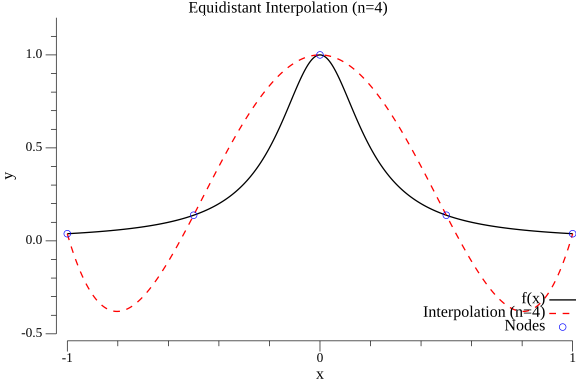
\includegraphics[width=1.0\linewidth]{material/runge/equidistant/runge_n04.png}
  \end{minipage}
  \hfill
  \begin{minipage}[b]{0.48\linewidth}
    \centering
    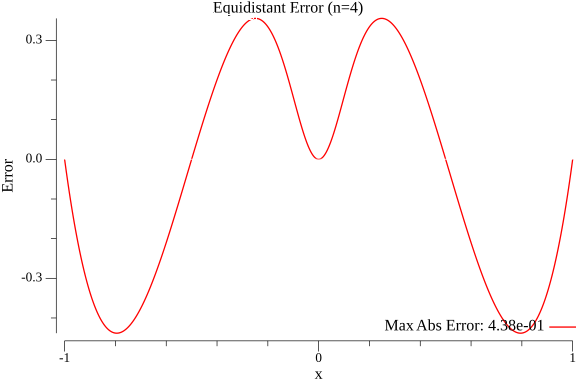
\includegraphics[width=1.0\linewidth]{material/runge/equidistant/runge_err_n04.png}
  \end{minipage}
\end{figure}

\begin{figure}[H]
  \centering
  \caption{$f(x) = \frac{1}{1+25x^2}$の等間隔補間（$n=7$次多項式）}
  \label{fig:runge-equidistant-2}
  \vspace{5pt}
  \begin{minipage}[b]{0.48\linewidth}
    \centering
    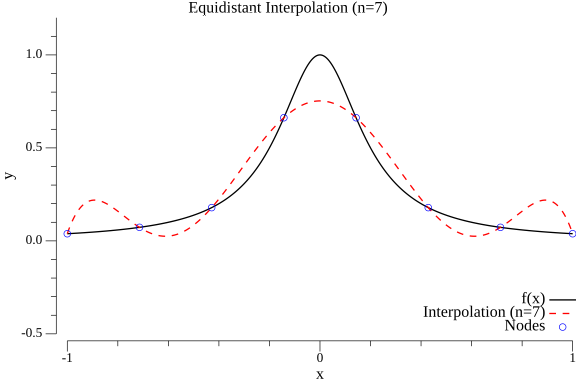
\includegraphics[width=1.0\linewidth]{material/runge/equidistant/runge_n07.png}
  \end{minipage}
  \hfill
  \begin{minipage}[b]{0.48\linewidth}
    \centering
    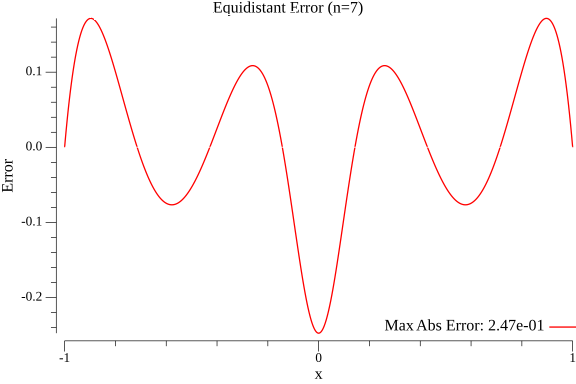
\includegraphics[width=1.0\linewidth]{material/runge/equidistant/runge_err_n07.png}
  \end{minipage}
\end{figure}

\begin{figure}[H]
  \centering
  \caption{$f(x) = \frac{1}{1+25x^2}$の等間隔補間（$n=15$次多項式）}
  \label{fig:runge-equidistant-last}
  \vspace{5pt}
  \begin{minipage}[b]{0.48\linewidth}
    \centering
    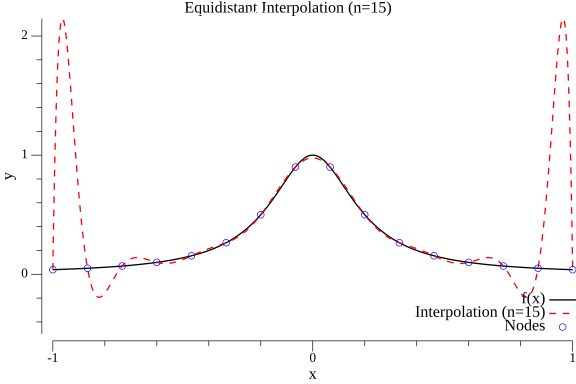
\includegraphics[width=1.0\linewidth]{material/runge/equidistant/runge_n15.png}
  \end{minipage}
  \hfill
  \begin{minipage}[b]{0.48\linewidth}
    \centering
    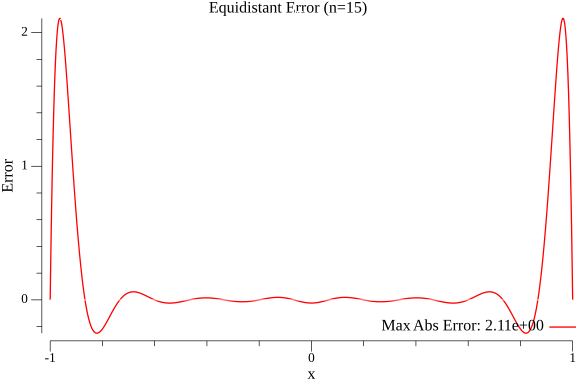
\includegraphics[width=1.0\linewidth]{material/runge/equidistant/runge_err_n15.png}
  \end{minipage}
\end{figure}

